\section{Conception d'un langage approprié}

Le langage développé reprend le cœur du lambda-calcul polymorphe
\cite{Reynolds94anintroduction} (aussi connu sous le nom de \emph{Système F})
et l'étend avec les notions de primitives et de \emph{bloc} muni d'un
\emph{tag} et les constructions d'analyse de tag et d'aiguillage.

Présentons tout d'abord le noyau de ce langage.

\subsection{Lambda-calcul polymorphe} 

Les trois premières constructions du langage sont les variables, l'application
et l'abstraction. Elles forment lambda-calcul simplement typé.

Ces trois constructions permettent de construire et d'appliquer des fonctions,
dont le type est noté par une \emph{flèche} paramétrée par le domaine et le
codomaine de la fonction.

L'application et l'abstraction de types rajoutent le polymorphisme, représenté
au niveau des types par la quantification universelle.

Contrairement à un langage tel qu'OCaml, la généralisation et l'instantiation
des valeurs polymorphes sont marquées explicitement. Si un tel langage devait
être utilisé dans le compilateur, c'est lors de la traduction que celles-ci
seraient ajoutées par le \emph{frontend}.

\subsection{Représentation des valeurs d'OCaml}

Les extensions ont été conçues autour de la représentation des valeurs par
OCaml. Les valeurs concrètes sont :
\begin{itemize}
  \item soit des entiers, directement représenté par un scalaire,
  \item soit des blocs représentés par un pointeur vers une
zone mémoire composée d'un \emph{tag} et d'un vecteur de valeurs.
\end{itemize}
Un bit des valeurs est réservé pour distinguer les entiers des pointeurs.

\begin{figure}
\centering
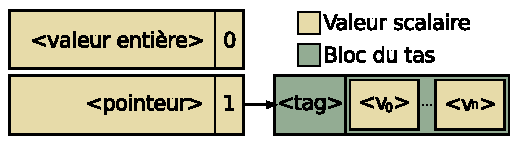
\includegraphics{media/ocaml_value}
\caption{Forme des valeurs}
\end{figure}

\paragraph{Types algébriques}

La spécificité de ML qui marque sans doute le plus ceux qui aprennent ce langage
sont les \emph{types sommes}. Les types de cette forme ont plusieurs
constructeurs de valeurs.

Ce comportement rappelle les \emph{union}s du C, mais les constructeurs des
types sommes sont disjoints : une fois construit, on peut retrouver sans
ambiguité le constructeur qui a engendré une valeur. Enfin, ces constructeurs
peuvent recevoir des paramètres. 

\begin{lstlisting}
  type address =
    | Any
    | Localhost
    | IP of int * int * int * int
    | Host of string

  let resolve addr = match addr with
    | Any -> 0, 0, 0, 0
    | Localhost -> 127, 0, 0, 1
    | IP (a,b,c,d) -> a, b, c ,d
    | Host host -> (* getaddrinfo ... *)
\end{lstlisting}

Ici, \emph{Any} est constant : il n'existe qu'une seule valeur de type
\emph{address} issue de ce constructeur. De même pour \emph{Localhost}, mais
cette unique valeur est différente de celle d'\emph{Any}. \emph{IP} et
\emph{Host} sont paramétrés.  L'analyse des constructeurs paramétrés constitue
un mécanisme sûr et vérifiable pour transporter des valeurs de différents types.

Les constructeurs constants sont encodés par des entiers, les constructeurs
paramétrés par un bloc de même arité.

La valeur des entiers et le tag des blocs servent à discriminer les différents
constructeurs durant le \emph{filtrage de motif}. Les entiers endossent ainsi
le même rôle que le \emph{tag} des blocs; ceux-ci sont testés dynamiquement
pour choisir un branchement.

L'encodage du type \emph{address} est le suivant :
\begin{description}
  \item[Any] l'entier 0
  \item[Localhost] l'entier 1
  \item[IP] un bloc de tag 0 et d'arité 4
  \item[Host] un bloc de tag 1 et d'arité 1
\end{description}

\paragraph{Variants polymorphes} 
Les variants polymorphes sont une forme plus souple de types sommes. En
particulier, ils ne nécessitent pas de déclarations préalables et peuvent
s'étendre. Dans l'analyse d'une de ces valeurs, cela se matérialise par la
présence de cas « par défaut ».

L'encodage ressemble à celui des types sommes, mais le \emph{tag} pour
discriminer les constructeurs paramétrés n'est plus celui du bloc. Une
indirection est ajoutée sous la forme d'un premier bloc composé du \emph{tag}
et d'un pointeur vers un n-uplet contenant les paramètres.

Du point de vue du langage intermédiaire, le \emph{tag} devient ici une valeur
de première classe, manipulable dans le langage.  En particulier, celui-ci
peut-être testé et transformé par l'application d'opérateurs.

\begin{figure}
\centering
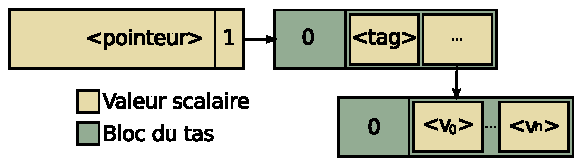
\includegraphics{media/ocaml_variant}
\caption{Forme des variants polymorphes}
\end{figure}

\subsection{Séparer extraction et analyse d'un \emph{tag}}

La principale contribution réside entre la séparation du calcul d'un tag et du
branchement qui s'ensuivra.

\paragraph{Filtrage de motif} Le \emph{filtrage de motif} est la construction
qui permet l'analyse des valeurs de types sommes pour sélectionner une branche
d'exécution.

Les différents constructeurs d'un type algébrique mènent chacun à une branche
différente. Dans chacune, des noms liés aux paramètres du constructeur
testé sont introduits. Le programmeur n'indique jamais explicitement l'accès
aux champs d'une valeur. Il ne peut même pas nommer un champ en dehors de la
branche.

Il est alors simple de vérifier l'exhaustivité du traitement et de garantir
l'absence d'accès à des valeurs inexistantes lors de l'exécution. Enfin le
compilateur se voit offrir beaucoup de libertés pour générer du code efficace,
différentes méthodes sont étudiées dans \cite{LeFessant:2001:OPM:507669.507641}
puis \cite{Maranget:2008:CPM:1411304.1411311}.

\paragraph{Motifs compilés} Le compilateur OCaml choisit de compiler ces motifs
très tôt. Dans le langage \emph{Lambda} il n'existe déjà plus que deux formes
de tests, les \emph{switch} et \emph{if} que l'on retrouve dans les langages
impératifs classiques. Une forme spécialisée de branchement proche du
\emph{goto} est aussi proposée pour factoriser le code des branches.

Les filtrages de haut-niveau sont ainsi traduits via des arbres de décisions,
au travers d'une suite de tests et de tables de sauts.  Le lien entre la
sélection d'une branche et les hypothèses qui y ont amené disparaît -- le
compilateur ne peut que suivre les instructions de projection sous l'hypothèse
que le code traduit est correct.

Voici le corps de la forme compilée de la fonction \emph{resolve} définie
ci-dessus :

\lstset{language=Lisp}
\begin{lstlisting}
(switch* addr
   ;; Any
   case int 0: [0: 0 0 0 0]
   ;; Localhost
   case int 1: [0: 127 0 0 1]
   ;; IP
   case tag 0:
    (makeblock 0 (field 0 addr) (field 1 addr)
      (field 2 addr) (field 3 addr))
   ;; Host
   case tag 1: ...)
\end{lstlisting}
\lstset{language=Caml}

Le lien entre une branche et la sélection qui y a mené est devenu implicite.
En particulier les projections dans la branche "IP", matérialisée par la
primitive \emph{field}, sont impossibles à vérifier.

Notre travail sur \emph{Lambda} vise à justifier la compilation de ces motifs ;
pour cela il faudra être capable de corréler statiquement la valeur d'un tag et
le type de la valeur \emph{taguée}.
